\section{Results and Discussions}
\label{chap:results}

The results presented in this chapter are a selection of the observables 
that we want to use in the first publication, eventually a long paper will
include results as function of all variables. All results were extracted with the following DIS selection cuts: 
$Q^2$~$>$~$1$~GeV$^2$/c$^2$, $W$~$>$~$2$ GeV and $y<0.85$. To ensure that SIDIS 
factorization applies~\cite{Mulders:2000jt}, we are selecting events with 
$0.4$~$<$~$z$~$<$~$0.7$~\footnote{This cut is not applied for plots with results 
as a function of $z$.} based on the previously published results from 
\cite{Asaturyan:2011mq}. Moreover, this cut also ensures that we are measuring the 
leading hadron, and avoiding the high $z$ region, which might be contaminated by 
the decay products of the diffractive production of $\rho^0$. Finally, we are 
applying a cut on $x_F > 0$ to select the forward fragmentation region.

\subsection{Multiplicity Ratio}

\subsubsection{$A$ Dependence}
\label{sec:resA}

\begin{figure}[p]
\centering
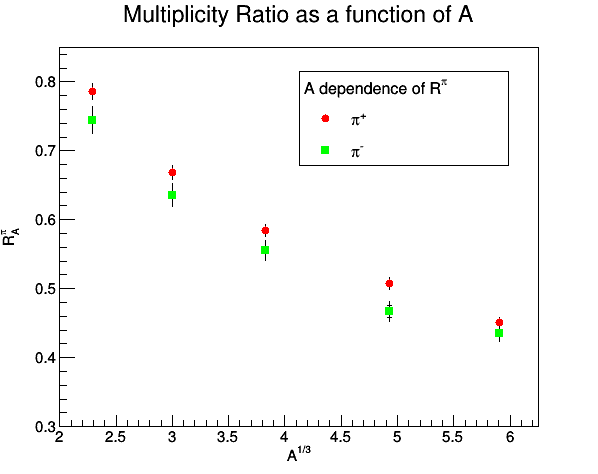
\includegraphics[width=7.4cm] {chap6-fig/F_RvA.png} 
\caption {$A^{1/3}$ dependence of the multiplicity ratio. Normalization 
uncertainties are not shown.}
\label{fig:RA}
\end{figure}

Figure \ref{fig:RA} contains our results for the $A^{1/3}$ dependence of 
the multiplicity ratio. One can see a 5\% normalization difference between both pions. However, this difference is not significant as it represents only 1.5 
standard deviation of our normalization uncertainty (see table~\ref{tab:sysid}).

The attenuation, presented in the figure \ref{fig:RA}, is neither linear as a 
function of $A^{1/3}$ nor as a function of $A^{2/3}$. The HERMES data had
already showed some indication 
of this feature~\cite{Airapetian:2007vu,Airapetian:2009jy}, but here the 
non-linearity, which has important implication on models, is clear. Indeed, 
it seems difficult to reconcile the prehadron absorption models with this result. Prehadrons 
are expected to have their cross sections increasing with time and, therefore, 
distance. On the parton energy loss side, the BDMPS calculation gives a parton 
energy loss proportional to $L^2 \propto A^{2/3}$, indicating that we are not
in the region where this result applies. Morover, if the production 
time\footnote{As defined in figure~\ref{fig:hadro}} occurs 
inside the nuclei, the behavior of the multiplicity ratio can be more complicated
as different processes intervene.

\subsubsection{Cronin Effect}

\begin{figure}[p]
\centering
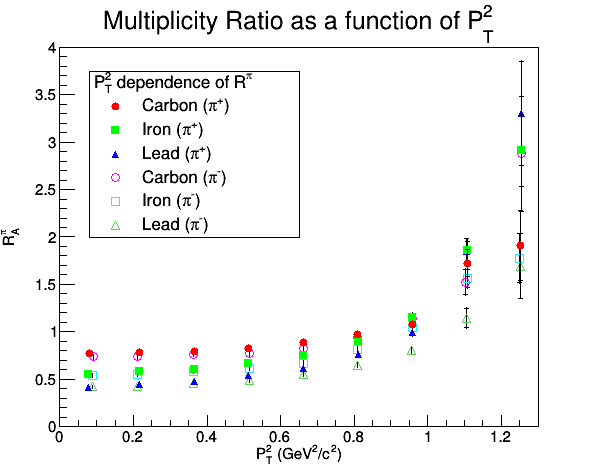
\includegraphics[width=7.4cm] {chap6-fig/F_RvPt.png} 
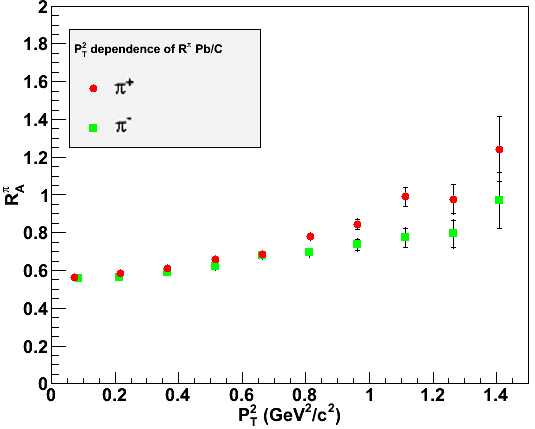
\includegraphics[width=7.4cm] {chap6-fig/F_RvPt_PbC.png} 
\caption {Multiplicity ratios as a function of \pt (GeV$^2$/c$^2$) for both charged pions. Left: The usual multiplicity ratio results. Right: Lead results normalized to carbon. Normalization uncertainties are not shown.}
\label{fig:RPt}
\end{figure}

\begin{figure}[p]
\centering
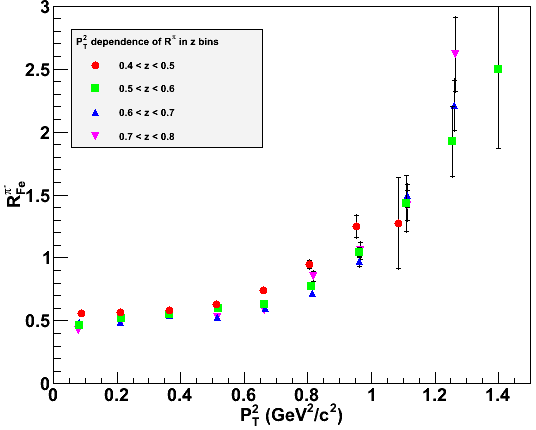
\includegraphics[width=7.4cm] {chap6-fig/F_RvPtinZ.png} 
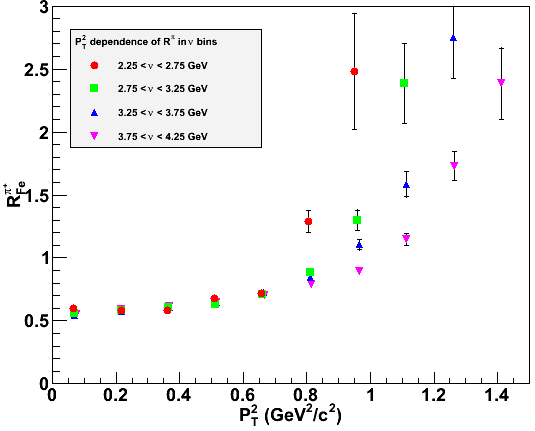
\includegraphics[width=7.4cm] {chap6-fig/F_RvPtinNu.png} 
\caption {Positive pions multiplicity ratios as a function of \pt (GeV$^2$/c$^2$) for different $z$ bins (left), and different $\nu$ (GeV) bins (right). Normalization uncertainties are not shown.}
\label{fig:RPtMulti}
\end{figure}

The Cronin effect is characterized by a large increase of the multiplicity 
ratio at high \pt ($\sim$1~GeV$^2$/c$^2$), which is a controversial result in hadronization studies. Indeed, whereas SLAC measurements 
\cite{Osborne:1978ai} did not show such an effect, HERMES \cite{Airapetian:2007vu} measured a significant increase of the multiplicity 
ratio with \ptp. Our result (figure \ref{fig:RPt} (left)), integrated over 
all other variables, showed a pattern similar to the HERMES measurement. 
However, there are some potential contributions from the target fragmentation and 
the Fermi motion.

Fermi motion effects can be significantly reduced by modifying our regular observables. Indeed, using carbon for normalization, instead of deuterium, most effects of Fermi motion cancel out. Moreover, acceptance effects (section~\ref{sec:accept}) will also be mostly canceled in such a ratio, leading to a reduction of their systematic errors dominated mainly by the normalization error. The normalized lead multiplicity ratio to carbon is presented on figure \ref{fig:RPt} (right). There is an attenuation, at low \ptp, similar to the usual multiplicity ratio of iron. This can be understood based on the difference of both nuclei radii, $R_{Pb}-R_{C} \sim R_{Fe}$. Nevertheless, the observed enhancement with \pt is much more modest than in iron. At first sight the difference can be attributed to Fermi motion, which might affect the normalized measurement with deuterium compared to carbon.

In figure \ref{fig:RPtMulti}, the multi-dimensional multiplicity ratio results are presented. HERMES found an important $z$ dependence of the Cronin effect \cite{Airapetian:2007vu,Airapetian:2011jp}. That can be treated as a sign of an essential contribution from a target fragmentation. The present result 
(figure~\ref{fig:RPtMulti} (left)) does not show this behavior, which could be due to our strict cut on $z$ ($z>0.4$ whereas HERMES used $z>0.2$) that leads to a smaller target fragmentation contamination. The second result, binned in \pt and $\nu$ (figure \ref{fig:RPtMulti} (right)), showed an important 
$\nu$ dependence of the Cronin effect. However, HERMES results did not exhibit such a $\nu$ behavior. This is a clear evidence of the importance of 
the Fermi motion effect in our measurement.

The result of the lead to carbon multiplicity ratio, figure \ref{fig:RPt} 
(right), has another interesting feature: the $\pi^+$s have a stronger Cronin 
effect. However, the significance of this observation is not clear. This could be 
a contribution from target fragmentation, as we might expect more positive 
particles would originate from nuclei than negative ones. This could also come from other sources such as the isospin effect or a factorization breaking at high 
\ptp. However, no test of these features exists in our kinematical range\footnote{Results of \cite{Asaturyan:2011mq} covered only \pt$<0.2$ GeV$^2$/c$^2$.}. Last but not least, it could be correlated with the hadronic rank and reflect some hadronization properties. Indeed, as we probe mostly valence quarks at our energies, $\pi^+$s are more likely to be the leading hadrons compared to $\pi^-$s.

In conclusion, our results indicate that the HERMES results were affected by a target fragmentation and that our results are affected by the Fermi motion. These effects can be easily controlled by a careful selection of our observables. In this regard, the Pb/C ratio seems to give cleaner results than Fe/D.

\subsubsection{$\nu$ Dependence}

\begin{figure}[tbp]
\centering
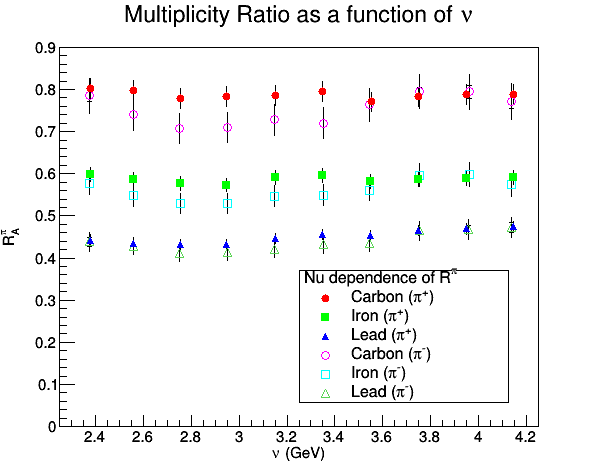
\includegraphics[width=7.4cm] {chap6-fig/F_RvNu.png} 
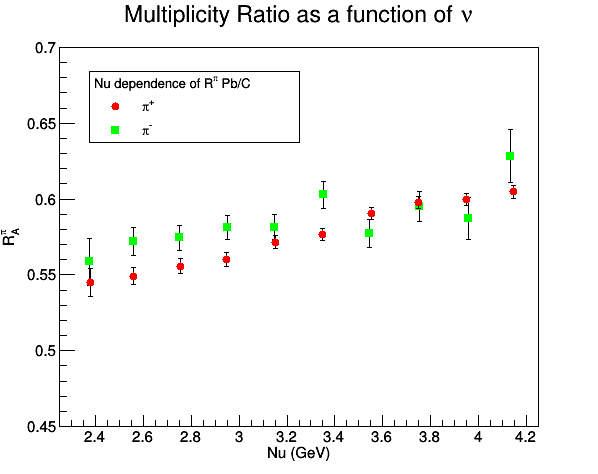
\includegraphics[width=7.4cm] {chap6-fig/F_RvNu_PbC.png} 
\caption{Multiplicity ratios as a function of $\nu$ (GeV) for both charged pions. Left: The usual multiplicity ratio results. Right: Lead results normalized to carbon. Normalization uncertainties are not shown.}
\label{fig:RNu}
\end{figure}

The HERMES collaboration clearly observed a rise of the multiplicity ratio 
with $\nu$ from 6 to 22~GeV. However, our results (figure \ref{fig:RNu} (left))
show no dependence, besides a slight increase in lead.
However, the Fermi motion could cancel most of this hadronization effect, and 
what is left will be washed out with the acceptance correction systematic 
uncertainty. The normalized multiplicity ratio to carbon offers a 
cleaner result, that is not affected by Fermi motion or acceptance. For this
observable, we measure a slope consistent with what was observed by HERMES.

We must note the similar behavior of both pions results in a figure 
\ref{fig:RNu} (right). This confirms our previous remark that the difference 
observed in the regular multiplicity ratio might originate from the 
normalization uncertainty caused by the acceptance correction. Also, there is no 
clear difference between both charged pions on the integrated multiplicity 
ratios as a function of $\nu$.

\subsubsection{$z$ Dependence}

\begin{figure}[tbp]
\centering
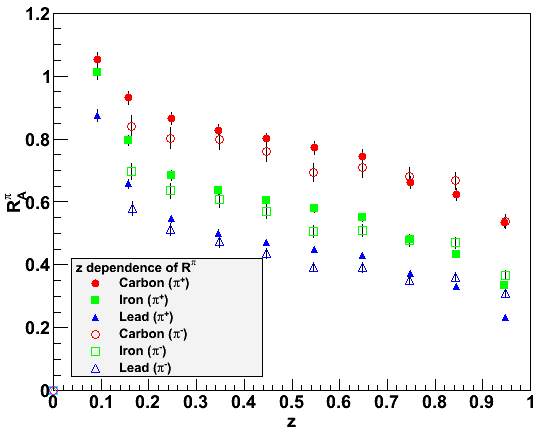
\includegraphics[width=7.4cm] {chap6-fig/F_RvZ.png} 
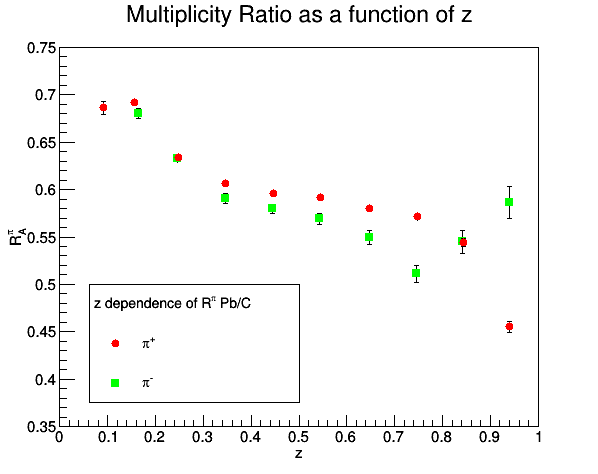
\includegraphics[width=7.4cm] {chap6-fig/F_RvZ_PbC.png} 
\caption {Multiplicity ratios as a function of $z$ for both charged pions. Left: The usual multiplicity ratio results. Right: Lead results normalized to carbon. 
Normalization uncertainties are not shown.}
\label{fig:Rz}
\end{figure}

The multiplicity ratio was observed to decrease with $z$ in HERMES data, 
whereas this behavior was not significant in other experiments. Indeed the 
nature of this behavior is questionable as the target fragmentation also get reduced 
with $z$, hence can mimic the signal. In figure \ref{fig:Rz} (left), as for HERMES results, we see a clear slope even at values higher than 0.4, where target fragmentation effects are expected to be small. However, the lead to carbon ratio (figure \ref{fig:Rz} (right)) shows a much flatter behavior in the region of interest (from 0.4 to 0.7). Therefore, this situation seems similar to the Cronin effect, where HERMES observation was enhanced by a target fragmentation. The measurement using the carbon as a basis is, therefore, more useful on isolating effects from the hadronization. However, the low $z$ behavior remains driven by the target fragmentation region. Another strange feature of the data is the behavior at higher $z$ (figure \ref{fig:Rz} (right)), where the two pions behave differently. However, there is a lack of solid theoretical grounds in this region to interpret this result.

\subsubsection{$Q^2$ Dependence}

The behavior of hadronization as a function of $Q^2$ is an important issue, that 
has direct implications on our understanding of nuclear matter properties in 
QCD. HERMES results, which covered $1<Q^2<10$~GeV$^2$/c$^2$, gave a hint of an 
increase of the multiplicity ratio with $Q^2$. Our result, in figure 
\ref{fig:RQ2}, does not indicate any $Q^2$ dependence, hence our 
conclusion is that the multiplicity ratio has no significant $Q^2$ dependence.

\begin{figure}[tbp]
\centering
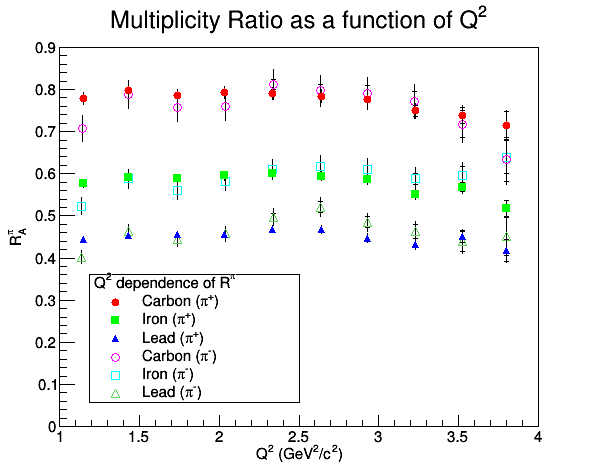
\includegraphics[width=7.4cm] {chap6-fig/F_RvQ2.png} 
\caption {Multiplicity ratios as a function of $Q^2$ (GeV$^2$/c$^2$). 
Normalization uncertainties are not shown.}
\label{fig:RQ2}
\end{figure}

We can use our large statistics to extract more information by handling the results differently. As a $\nu$ dependence is expected for the multiplicity ratio, it might be helpful to use a tighter $\nu$ bin to plot the $Q^2$ dependence (figure \ref{fig:RQ2Detailed} (left)), thus remove any coupling between the two variables.
As some Fermi motion effects would persist, it is more convenient to show the $Q^2$ dependence of the normalized multiplicity ratio of lead to carbon, see figure \ref{fig:RQ2Detailed} (right). The two results of figure \ref{fig:RQ2Detailed} 
showed a slight increase with $Q^2$, but as for HERMES, no evidence is 
reached on this context. Our leverage on $Q^2$ appears to be too modest to make a clear measurement. 

\begin{figure}[tbp]
\centering
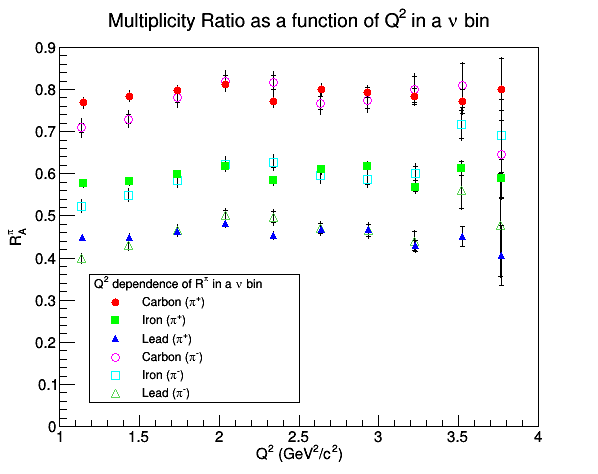
\includegraphics[width=7.4cm] {chap6-fig/F_RvQ2inNu.png} 
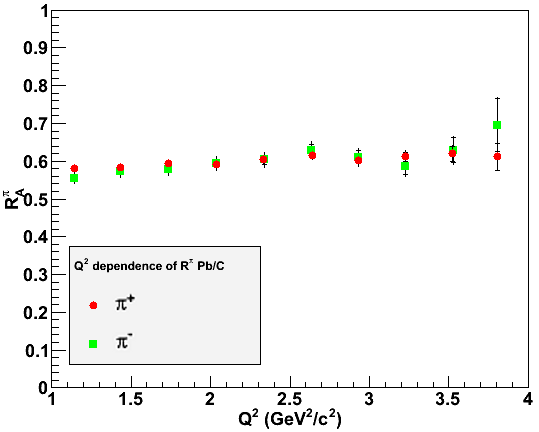
\includegraphics[width=7.4cm] {chap6-fig/F_RvQ2_PbC.png} 
\caption {Multiplicity ratios as a function of $Q^2$ (GeV$^2$/c$^2$) for both charged pions. Left: The multiplicity ratio for a tighter $\nu$ bin ($3.25 < \nu < 3.75$ GeV). Right: The normalized multiplicity ratio of lead to carbon. Normalization uncertainties are not shown.}
\label{fig:RQ2Detailed}
\end{figure}

\subsection{Transverse Momentum Broadening}

\subsubsection{$A$ Dependence}

The $A$ dependence of the transverse momentum broadening, presented in 
figure~\ref{fig:PA}, is a crucial result. The combination of our large 
statistics with a wide $A$ coverage gives an outright indication of $A^{1/3}$ 
dependence of \dpt. This \dpt effect is found to be much smaller than that seen 
by HERMES\cite{Airapetian:2009jy}, which is consistent with
 theoretical models predicting larger effects at larger energies. However, 
calculations of the parton energy loss from BDMPS \cite{Baier:1996sk} 
correlated \pt with the square of the nuclear radius. A feature that is not 
observed in our result. Although, by looking to the low energy of our CLAS 
experiment, one might argue the validity of a direct comparison with BDMPS 
calculations. Nonetheless, this result shows an unexpected pattern that 
remains to be explained. One possible interpretation is the occurrence of 
the production time inside the nuclei, as we proposed for the $A^{1/3}$ 
dependence of multiplicity ratios. In this case, the colored parton does 
not interact with the whole nucleus which limits the nuclear effect.

\begin{figure}[tbp]
\centering
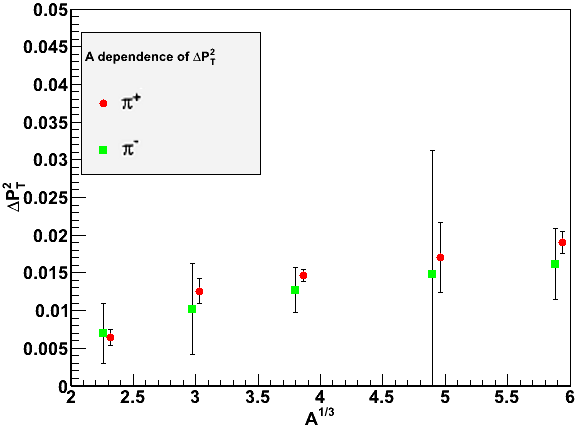
\includegraphics[width=8.2cm] {chap6-fig/F_PvA.png} 
\caption {$A$ dependence of \dptp. Points are slightly shifted for a readability. Normalization uncertainties are not shown.}
\label{fig:PA}
\end{figure}

\subsubsection{$Q^2$ Dependence}

Finally, the $Q^2$ dependence of \dpt is an important result for the BDMPS based 
calculation from \cite{Domdey:2008aq}. They predict a raise of \dpt with $Q^2$, 
which is not observed in figure \ref{fig:PQ2}. Using a tighter $\nu$ bin and a 
carbon normalization should isolate this effect better, but figure \ref{fig:PQ2-detailed}
gives a similar result. In conclusion, within error bars, no effect is observed for 
\dpt as a function of $Q^2$. However, we would like to have a quantitative theoretical 
input here, as it is not clear if we have the needed resolution to observe the effect 
expected within BDMPS based models. We are going to work with the authors of the original 
paper to add some projections on our figures.

\begin{figure}[tbp]
\centering
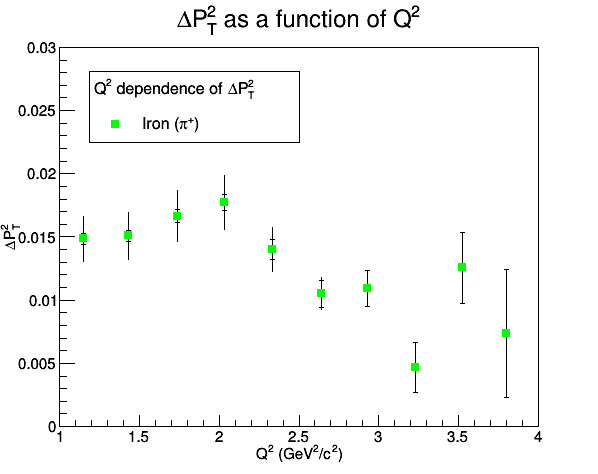
\includegraphics[width=7.4cm] {chap6-fig/F_PvQ2.png} 
\caption {Iron \dpt as a function of $Q^2$ (GeV$^2$/c$^2$) after applying the regular DIS cuts. Normalization uncertainties are not shown.}
\label{fig:PQ2}
\end{figure}

\begin{figure}[tbp]
\centering
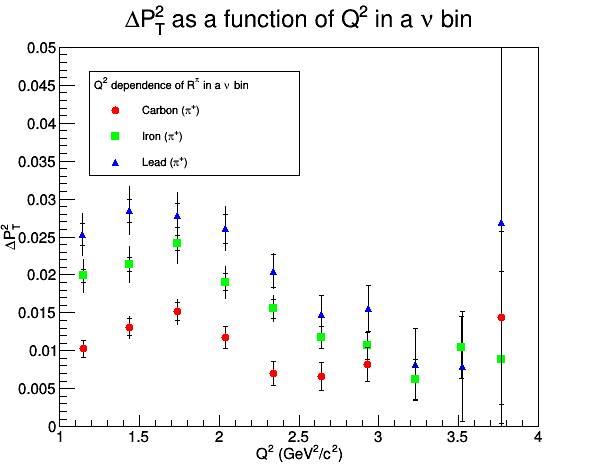
\includegraphics[width=7.4cm] {chap6-fig/F_PvQ2inNu.png} 
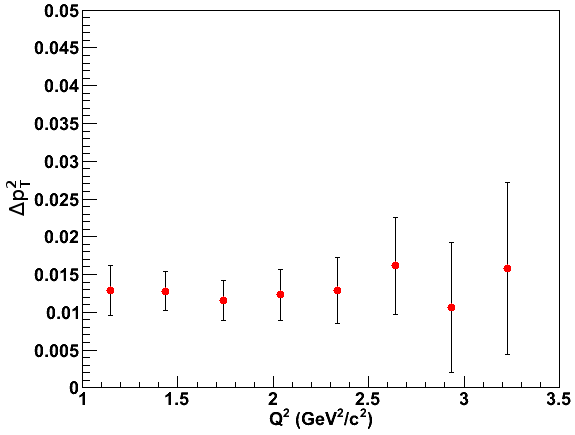
\includegraphics[width=7.4cm] {chap6-fig/F_PvQ2_PbC.png} 
\caption {Positive pions \dpt as a function of $Q^2$ (GeV$^2$/c$^2$). Left: The usual observable for a tighter $\nu$ bin ($3.25 < \nu < 3.75$~GeV). Right: \dpt 
of lead relative to carbon. Normalization uncertainties are not shown.}
\label{fig:PQ2-detailed}
\end{figure}

